\documentclass[12pt]{article}

\usepackage[margin=1in]{geometry}
\usepackage{amsmath,amsthm,amssymb,amsfonts,graphicx}
\usepackage{hyperref}

\newcommand{\Pp}{\emph{\emph{P}}}

\begin{document}

\title{Statistics Homework 4}
\author{Mr. Grant}
\maketitle

\textbf{Due Date:} Tuesday, July 18th \\

This homework can be done either by hand or on the computer. It will be \textbf{much} faster if you do it on the computer--trust me. If you do it on the computer, turn in a word document with the graphs pasted into it. If you do it by hand, you will have to draw the graphs neatly by hand. In either case,
\begin{itemize}
	\item Be neat
	\item Put your name, the date, and the name of this class on your homework 
	\item Number each problem clearly
	\item Show your work
\end{itemize}

These questions all use the data from \textit{class\_data\_complete.csv}.
\begin{enumerate}
	\item Make boxplots of the heights of the girls and the boys in the class (use the Shoe Gender variable to determine gender). Put the boxplots on the same graph, so that you can compare the boys to the girls easily. We will learn how to do this in R on Wednesday (or you can Google it!).
	\item What do the boxplots tell you about the height of the average woman in the class versus the height of the average man? Why? Which gender has more variability in height, and how can you tell from the boxplot? We already know the answers to these questions from class, so your explanation of how you can tell from the boxplot is what matters.
	\item Suppose Booker randomly picks a girl in the class to go on a date with. What is the probability that she is 5'4" or shorter? What is the probability that she is taller than 5'8"? \textbf{Given that he has picked a girl who is 5'5" or taller}, what is the probability that Booker chose Idara? What is the probability that Booker goes on a date with a Hawaiian who is exactly five feet tall?
	\item Consider the boxplot you made in question 1 and answer the following true/false questions. With each question, give a 1-sentence explanation of why you know your answer is correct.
	\begin{itemize}
		\item The tallest $\frac{3}{4}$ of the boys in the class are taller than the shortest $\frac{3}{4}$ of the girls.
		\item If Idara were a boy, she would be shorter than Q3.
		\item If Pearson were a girl, he would be an outlier.
	\end{itemize}
\item Read \href{https://www.insidehighered.com/news/2017/04/26/college-completion-rates-vary-race-and-ethnicity-report-finds}{this} article and answer the following questions:
	\begin{itemize}
		\item Which is more likely--a white student getting a degree from the college they started at in 6 years, or a black student getting a degree from any university in 6 years? 
		\item Approximately how many--not what percent, but how many--eligible Asian students did not enroll in college in 2010 (the number of students of each race is shown at the bottom of the graph; for example, there were 322,205 Hispanic students in this study)? 
		\item Do you think the percentages in this study are likely to apply to STEMPrep students? Why or why not?
	\end{itemize}
\end{enumerate}


\begin{enumerate}
	\item 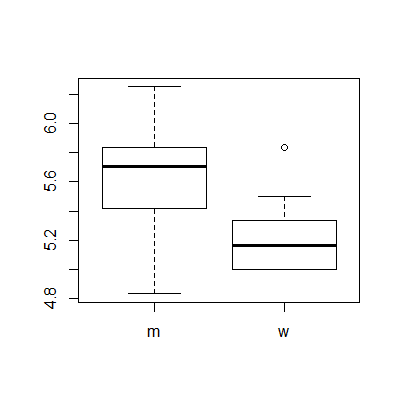
\includegraphics{hw5boxplot}
	\item We can from the bold black line that the median height of the boys is around 5.7 ft, whereas for girls it is about 5.2 ft. Furthermore, the first quartile of boys' heights is taller than the third quartile of girls' heights. These both indicate that boys are taller than girls on average. The boys' heights appear to be more variable, as well. The range of heights is much larger for boys: their heights run from about 4.8 ft to 6.3 ft, whereas the girls' heights only run from 5 ft to 5.8 ft. The ``box'' in the boxplot is a bit bigger for boys than girls, as well.
	\item See attached code. The probability of a girl 5'4" or shorter is the number of girls 5'4" or shorter divided by the total number of girls, which is .764. The probability of a girl taller than 5'8" is, similarly (see how these first two questions are basically the same question because they require the exact same kind of reasoning), .058. The third part is a conditional probability: we count the number of Idaras (just one, sadly) and divide by the condition: the number of girls 5'5" or taller. That gives us 0.25. For the final part, we need to count the number of people who are girl, Hawaiian, and exactly 5 feet. We can use 3 conditions and put them together with ``and'' symbols (see code) to get a probability of .176.
	\item
		\begin{enumerate}
			\item Yes--the whole boys' box is taller than the whole girls' box.
			\item It looks like Idara would be 
		\end{enumerate}
\end{enumerate}

\end{document}
